\documentclass[10pt, a5paper]{article}
\usepackage{pdfpages}
\usepackage{parallel}
\usepackage[T2A]{fontenc}
\usepackage{ucs}
\usepackage[utf8x]{inputenc}
\usepackage[polish,english,russian]{babel}
\usepackage{hyperref}
\usepackage{rotating}
\usepackage[inner=2cm,top=1.8cm,outer=2cm,bottom=2.3cm,nohead]{geometry}
\usepackage{listings}
\usepackage{graphicx}
\usepackage{wrapfig}
\usepackage{longtable}
\usepackage{indentfirst}
\usepackage{array}
\newcolumntype{P}[1]{>{\raggedright\arraybackslash}p{#1}}
\frenchspacing
\usepackage{fixltx2e} %text sub- and superscripts
\usepackage{icomma} % коскі ў матэматычным рэжыме
\PreloadUnicodePage{4}

\newcommand{\longpage}{\enlargethispage{\baselineskip}}
\newcommand{\shortpage}{\enlargethispage{-\baselineskip}}

\def\switchlang#1{\expandafter\csname switchlang#1\endcsname}
\def\switchlangbe{
\let\saverefname=\refname%
\def\refname{Літаратура}%
\def\figurename{Іл.}%
}
\def\switchlangen{
\let\saverefname=\refname%
\def\refname{References}%
\def\figurename{Fig.}%
}
\def\switchlangru{
\let\saverefname=\refname%
\let\savefigurename=\figurename%
\def\refname{Литература}%
\def\figurename{Рис.}%
}

\hyphenation{admi-ni-stra-tive}
\hyphenation{ex-pe-ri-ence}
\hyphenation{fle-xi-bi-li-ty}
\hyphenation{Py-thon}
\hyphenation{ma-the-ma-ti-cal}
\hyphenation{re-ported}
\hyphenation{imp-le-menta-tions}
\hyphenation{pro-vides}
\hyphenation{en-gi-neering}
\hyphenation{com-pa-ti-bi-li-ty}
\hyphenation{im-pos-sible}
\hyphenation{desk-top}
\hyphenation{elec-tro-nic}
\hyphenation{com-pa-ny}
\hyphenation{de-ve-lop-ment}
\hyphenation{de-ve-loping}
\hyphenation{de-ve-lop}
\hyphenation{da-ta-ba-se}
\hyphenation{plat-forms}
\hyphenation{or-ga-ni-za-tion}
\hyphenation{pro-gramming}
\hyphenation{in-stru-ments}
\hyphenation{Li-nux}
\hyphenation{sour-ce}
\hyphenation{en-vi-ron-ment}
\hyphenation{Te-le-pathy}
\hyphenation{Li-nux-ov-ka}
\hyphenation{Open-BSD}
\hyphenation{Free-BSD}
\hyphenation{men-ti-on-ed}
\hyphenation{app-li-ca-tion}

\def\progref!#1!{\texttt{#1}}
\renewcommand{\arraystretch}{2} %Іначай формулы ў матрыцы зліпаюцца з лініямі
\usepackage{array}

\def\interview #1 (#2), #3, #4, #5\par{

\section[#1, #3, #4]{#1 -- #3, #4}
\def\qname{LVEE}
\def\aname{#1}
\def\q ##1\par{{\noindent \bf \qname: ##1 }\par}
\def\a{{\noindent \bf \aname: } \def\qname{L}\def\aname{#2}}
}

\def\interview* #1 (#2), #3, #4, #5\par{

\section*{#1\\{\small\rm #3, #4. #5}}

\def\qname{LVEE}
\def\aname{#1}
\def\q ##1\par{{\noindent \bf \qname: ##1 }\par}
\def\a{{\noindent \bf \aname: } \def\qname{L}\def\aname{#2}}
}

\begin{document}
\title{Технология прозрачного сжатия графической памяти GPU}
\author{Сергей Рогачев, Москва, Russian Federation}
\maketitle
\begin{abstract}
Complexity of graphical user interfaces of mobile applications is growing rapidly. Much memory is needed to keep buffers for textures and graphical data. Modern mobile GPUs do not have built-in memory and use general memory to keep graphic buffers. A part of RAM is occupied by GPU and cannot be used by an operating system. According to this research most of such buffers are well compressible: 6-9 times. We propose a technology for transparent compression of graphic buffers in Linux kernel.
\end{abstract}
Каждый год анонсируются новые, все более совершенные гаджеты, использующие ядро Linux и открытые платформы: планшеты, смартфоны, телевизионные приставки, умные часы. Большинство из них оснащается мобильными GPU, используемыми для аппаратного ускорения 3D графики (OpenGL ES) и параллельных вычислений (OpenCL, RenderScript). Наиболее часто встречаются графические процессоры Mali, Adreno и PowerVR. В отличие от GPU, используемых в настольных системах, мобильные GPU не имеют встроенной памяти, а используют часть оперативной (рис. ~\ref{Rogachev1}), предоставляемой ядром ОС "--- такая память становится недоступной ядру ОС и пользовательским программам. Будем называть память, используемую GPU, графической памятью. Оптимизация расхода такой памяти позволит достичь снижения цены устройств или повысить производительность за счет улучшения кешируемости приложений.

\begin{figure}[h!]
  \centering
  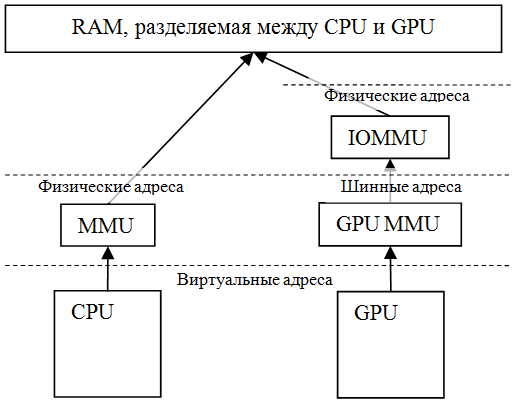
\includegraphics[]{18_2016_Rogachev1.png}
  \caption{Разделение памяти между CPU и GPU}
  \label{Rogachev1}
\end{figure}

К графической памяти можно отнести GEM буферы, используемые для хранения результата рендеринга, и вспомогательные регионы (native буферы), хранящие цветовые буферы, поверхности, текстуры, различную вспомогательную информацию, относящуюся к элементам графической сцены.

Задача оптимизации использования графической памяти уже рассматривалась ранее ~\cite{Rogachev1}, в статье упоминалась технология сжатия GEM буферов на стороне пользователя, также были отмечены высокие накладные расходы этого решения.

В настоящей работе рассматривается исключительно вопрос оптимизации использования native буферов, поскольку современные композитные менеджеры уже способны эффективно управлять \linebreak GEM буферами и дальнейшая работа в этом направлении не требуется.

Авторами было проведено исследование вопроса на примере \linebreak GPU Mali серий Midgard и Utgard: за счет доработки драйверов ядра удалось реализовать прозрачную компрессию редко используемых native буферов графической памяти. В результате получилось добиться экономии более 100 Мб. оперативной памяти за счет высокого коэффициента сжатия графических буферов (6 "--- 9 раз), а также наличия множества регионов графической памяти, заполненных нулями.

По своей сути решение реализует механизм схожий с подкачкой страниц (swap), при этом есть ряд особенностей, характерных для графической памяти и мобильных устройств. Ранее подобный подход рассматривался как трудно реализуемый ~\cite{Rogachev2}.

Для сжатия некоторого региона графической памяти нужна гарантия, что он не будет использоваться CPU или GPU в процессе компрессии. Это гарантируется путем запрета доступа к страницам данного региона в таблицах страниц GPU, а также снятия отображений региона в адресные пространства процессов на CPU. После того, как соответствующие записи PTE и ATE (записи таблиц страниц CPU и GPU, соответственно) изменены, любое обращение к соответствующим адресам памяти должно вызвать исключение страничной адресации, известное как page fault или data abort.

После того как гарантировано отсутствие доступа к региону памяти, данные со страниц этого региона могут быть сжаты, а страницы освобождены. Для хранения сжатых данных графической памяти в работе применена подсистема GMC (graphical memory compression), созданная в качестве обобщенного слоя для разных драйверов GPU. GMC осуществляет управление буферами для хранения сжатых данных через подсистему ядра zpool (zsmalloc \linebreak allocator ~\cite{Rogachev3}), сжатие данных с использованием crypto comp API, управление идентификаторами сжатых страниц, а также контролирует когерентность кешей. Страницы, данные которых плохо сжимаются, не принимаются для хранения и не освобождаются. Страницы, заполненные нулями, учитываются GMC и освобождаются.

При обращении к адресам страниц графической памяти, освобожденной ранее, генерируются исключения страничной адресации.  Соответствующие данные извлекаются из хранилища GMC на вновь выделенные страницы физической памяти. Осуществляется отображение новых страниц по требуемым виртуальным адресам путем изменения записей PTE или ATE в соответствующих таблицах страниц.

Кроме уже описанного механизма важным является вопрос о ранжировании регионов графической памяти по признаку частоты доступа. Сжатие активно используемой памяти может привести к катастрофическому падению производительности за счет частых исключений страничной адресации. Для решения указанной проблемы используется информация о состоянии приложений. Специальный демон (resource daemon) следит за приложениями и информирует ядро о тех из них, которые переходят в фоновый режим (становятся невидимыми на экране). Графическая память таких приложений подлежит сжатию.

Взаимодействие всех компонент во время компрессии отражено на рис. ~\ref{Rogachev2}. Основные шаги пронумерованы.

\begin{figure}[h!]
  \centering
  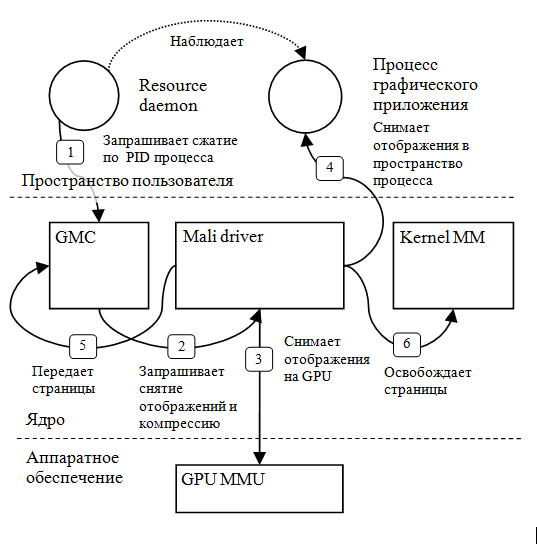
\includegraphics[]{18_2016_Rogachev2.png}
  \caption{Взаимодействие компонент системы}
  \label{Rogachev2}
  
\end{figure}

Рис. ~\ref{Rogachev3} иллюстрирует снятие отображений, компрессию и освобождение страниц с позиции данных, а не потока управления и дополняет рис. ~\ref{Rogachev2}.

\begin{figure}[h!]
  \centering
  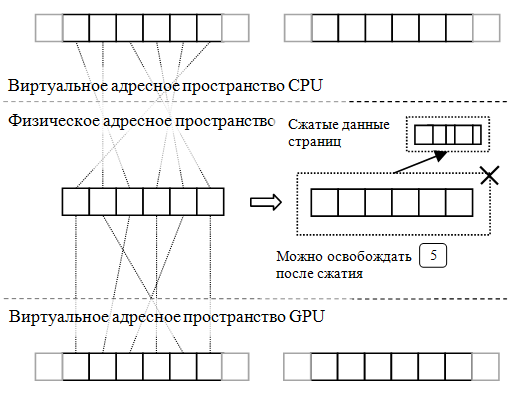
\includegraphics[]{18_2016_Rogachev3.png}
  \caption{Снятие отображений и компрессия}
  \label{Rogachev3}
\end{figure}

Тестирование решения на платформах Android и Tizen показало сокращение используемой памяти "--- более 100 мегабайт может быть освобождено при стандартном использовании устройства, когда в фоне оказывается достаточное количество кешированных приложений. Замечено большое количество регионов, заполненных нулями, а максимальная степень сжатия данных графических буферов составила 89\%. Накладные расходы, вносимые решением минимальны, а пиковые не превышают 18\% (Kindle App, Google Maps). В определенных ситуациях переключение между приложениями ускоряется до 40\% за счет большего количества свободной памяти, а следовательно, лучшей кешируемости приложений.

Исходный код подсистемы GMC планируется опубликовать в LKML, а изменения в драйверах Mali через группы поддержки ARM.

\begin{thebibliography}{99}
\bibitem{Rogachev1} Kwon, S., Kim, S.-H., Kim, J.-S., and Jeong, J. Managing gpu buffers for caching more apps in mobile systems. Proceeding EMSOFT '15, 207–216 (2015)
\bibitem{Rogachev2} Carmack, J. GPU data paging, \url{http://media.armadilloaerospace.com/misc/gpuDataPaging.htm} (2010)
\bibitem{Rogachev3} Corbet J. The ZsmallocAllocator. Linux Weekly News (2012)
\end{thebibliography}
\end{document}
